\id{МРНТИ \href{https://grnti.ru/?p1=06&p2=52&p3=13}{06.52.13}}

\begin{articleheader}
\sectionwithauthors{Х.Батцэнгэл, С.Б. Касымова, К.С. Мустафаев}{ҚАЗАҚСТАН РЕСПУБЛИКАСЫ ӨҢІРЛЕРІНІҢ ТҰРАҚТЫ ДАМУЫН ӘЛЕУМЕТТІК-ЭКОНОМИКАЛЫҚ БАҒАЛАУ}

{\bfseries ¹Х.Батцэнгэл\textsuperscript{\envelope }, ²С.Б. Касымова, ²К.С.
Мустафаев}
\end{articleheader}
\begin{affiliation}
¹Моңғол жоғары оқу орнынан кейінгі білім беру университеті, Ұлан-Батор,
Моңғолия,

²Қ.Құлажанов атындағы Қазақ технология және бизнес университеті, Астана,
Қазақстан

\raggedright {\bfseries \textsuperscript{\envelope }}Корреспондент-автор:\href{mailto:Sanim_81@list.ru}{\nolinkurl{Sanim\_81@list.ru}}
\end{affiliation}

Аймақтың тұрақты дамуы, ең алдымен, әлеуметтік-экономикалық және
табиғи-экологиялық даму факторлары арасындағы тепе-теңдікпен қамтамасыз
етіледі. Өңірдің орнықты дамуы, өздеріңіз білетіндей,
экологиялық-экономикалық және әлеуметтік факторларды теңгерімді
пайдалануды көздейді. Бұл ғылыми зерттеуде өңірлік экономика шеңберінде
тұрақты даму мақсаттарына қол жеткізудің негізгі тәсілдері
қарастырылады, өңірдің тұрақты дамуының негізгі анықтамалары зерделенеді
және тұрақты даму процестеріне әсер ететін факторлардың сипаттамасы
беріледі. Ғылыми жұмыстың мақсаты макроэкономикалық көрсеткіштерді
талдау негізінде Қазақстан Республикасы өңірлерінің тұрақты дамуы
контексінде қалыптасқан әлеуметтік\-экономикалық сәйкессіздіктерді
анықтау болып табылады. Аймақтардың тұрақты дамуға бейімделуін зерттеу
объектісі өңірдің әлеуметтік-экономикалық әлеуеті болып табылатындықтан,
оны пайдалану жалпы республика экономикасын реформалау барысымен
айқындалады, авторлар тұрақты дамуға бейімделудің өңірлік коэффициентін
есептеді. Өңірлердің орнықты даму талаптарына бейімделу дәрежесін
анықтау сандық және сапалық тәсілдерді біріктіруді талап ететін күрделі
мәселелердің бірі болып табылады. Зерттеу барысында тұрақты даму
тенденцияларын анықтауға мүмкіндік беретін экономикалық талдаудың
статистикалық және салыстырмалы әдістері қолданылды. Жүргізілген
экономикалық талдау негізінде теріс әсер ететін белгілі бір
теңгерімсіздіктер анықталды.

{\bfseries Түйін сөздер:} аймақ, тұрақты даму, әлеуметтік-экономикалық
даму, макроэкономикалық көрсеткіштер, тұрақтылық, бейімделудің аймақтық
коэффициенті.

\begin{articleheader}
{\bfseries СОЦИАЛЬНО-ЭКОНОМИЧЕСКАЯ ОЦЕНКА УСТОЙЧИВОГО РАЗВИТИЯ РЕГИОНОВ
РЕСПУБЛИКИ КАЗАХСТАН} 

{\bfseries ¹Х.Батцэнгэл\textsuperscript{\envelope }, ²С.Б. Касымова, ²К.С.
Мустафаев}
\end{articleheader}

\begin{affiliation}
¹Монгольский университет поствысшего образования, г. Улан-Батор,
Монголия,

²Казахский университет технологии и бизнеса имени К.Кулажанова, г.
Астана, Казахстан,

e-mail: \href{mailto:Sanim_81@list.ru}{\nolinkurl{Sanim\_81@list.ru}}
\end{affiliation}

Устойчивое развитие региона обеспечивается, прежде всего, равновесием
между факторами \\социально-экономического и природно-экологического
развития. Устойчивое развитие региона предполагает, как известно
сбалансированное использование эколого-экономических и социальных
факторов. В данном научном исследовании рассматриваются основные подходы
по достижению целей устойчивого развития в рамках региональной
экономики, изучены основные определения устойчивого развития региона и
дано описание факторов, оказывающих влияние на процессы устойчивого
развития. Цель научной работы состоит выявление сложившихся социально --
экономических диспропорций в контексте устойчивого развития регионов
Республики Казахстан на основе анализа макроэкономических показателей.
Поскольку объектом исследования адаптации регионов к устойчивому
развитию является социально-экономический потенциал региона,
использование которого определяется ходом реформирования экономики
республики в целом, авторами был рассчитан региональный коэффициент
адаптации к устойчивому развитию. Определение степени адаптации регионов
к требованиям устойчивого развития является одной из сложных проблем,
требующих сочетания как количественного, так и качественного подходов.
При исследовании были использованы статистический и сравнительный методы
экономического анализа, которые позволили выявить тенденции устойчивого
развития. На основе проведенного экономического анализа были выявлены
определенные дисбалансы, оказывающих негативное влияние.

{\bfseries Ключевые слова:} регион, устойчивое развитие,
социально-экономическое развитие, макроэкономические показатели,
стабильность, региональный коэффициент адаптации.

\begin{articleheader}
{\bfseries SOCIO-ECONOMIC ASSESSMENT OF SUSTAINABLE DEVELOPMENT OF REGIONS
OF THE REPUBLIC OF KAZAKHSTAN}

{\bfseries ¹K.Battsengel\textsuperscript{\envelope }, ²S.B. Kassymova, ²K.S.
Mustafaev}
\end{articleheader}

\begin{affiliation}
¹Graduate University of Mongolia, Ulanbaatar, Mongolia

²K.Kulazhanov Kazakh University of Technology and Business, Astana,
Kazakhstan,

e-mail: \href{mailto:Sanim_81@list.ru}{\nolinkurl{Sanim\_81@list.ru}}
\end{affiliation}

The sustainable development of the region is ensured, first of all, by
the balance between the factors of socio-economic and natural-ecological
development. Sustainable development of the region presupposes, as is
well known, a balanced use of environmental, economic and social
factors. This scientific study examines the main approaches to achieving
sustainable development goals within the framework of the regional
economy, examines the main definitions of sustainable development in the
region and describes the factors influencing the processes of
sustainable development. The purpose of the scientific work is to
identify the existing socio -- economic imbalances in the context of
sustainable development of the regions of the Republic of Kazakhstan
based on the analysis of macroeconomic indicators. Since the object of
the study of the adaptation of regions to sustainable development is the
socio-economic potential of the region, the use of which is determined
by the course of reforming the economy of the republic as a whole, the
authors calculated the regional coefficient of adaptation to sustainable
development. Determining the degree of adaptation of regions to the
requirements of sustainable development is one of the complex problems
that require a combination of both quantitative and qualitative
approaches. Statistical and \\comparative methods of economic analysis
were used in the study, which made it possible to identify trends in
sustainable development. Based on the conducted economic analysis,
certain imbalances have been identified that have a negative impact.

{\bfseries Keywords:} region, sustainable development, socio-economic
development, macroeconomic indicators, stability, regional coefficient
of adaptation.

\begin{multicols}{2}
{\bfseries Кіріспе.} Қазіргі кезеңде ұлттық экономиканы дамытудың аумақтық
факторлары күшейе түсуде. Бұл диспропорциялардан,
әлеуметтік-экономикалық дамудың әртүрлі деңгейлерінен, экономиканың тең
емес құрылымынан және аймақтық дамудағы мамандандырудан туындайды.
Өңірлердің дамуы тұтастай алғанда елдің дамуына әкелетіні белгілі.

Әлеуметтік-экономикалық жағдайдағы аймақтық айырмашылықтарды шамамен
объективті (аймақтың даму деңгейі, оның мамандануы мен экономиканың
құрылымы, экономикалық-географиялық жағдайы және басқалары) және
субъективті (барлық деңгейдегі билік органдарының саясаты) деп бөлуге
болады. Аймақтық даму тенденцияларын түсіну үшін осы факторлардың
заңдылықтарын, қатынастарын және әсер ету дәрежесін анықтау қажет.

Алайда, мұндай жұмыстарды жүргізу кезінде тұрақты дамуға бағытталған
аймақтық қайта құрулардың барысын барынша толық көрсететін «негізгі»
көрсеткішті анықтау қажет болады. Біз әлеуметтік даму деңгейі осындай
көрсеткіш ретінде қызмет ете алатын көзқараспен бөлісеміз, өйткені ол
барлық басқа көрсеткіштермен байланысты және аймақтарды реформалаудың
басты мақсаты болып табылады.

Егер ұлттық деңгейде мемлекет қызметінде әлеуметтік деңгеймен қатар
саяси, геостратегиялық, қауіпсіздік және басқа аспектілер болса, онда
аймақтық саясатта әлеуметтік аспект басым болады. Оның объектісі-өмір
сүру деңгейі мен жағдайындағы, жұмыспен қамту деңгейіндегі аймақаралық
теңсіздіктер, сондай-ақ экономикалық даму қарқынындағы, бизнес
жағдайындағы және т.б. аймақтар арасындағы айырмашылықтарды анықтайтын
факторлар. Алайда, мақсаттар теңдестірілген аймақтық саясатты әзірлеу
арқылы осы теңсіздіктерді азайту болып табылады.

Әлемнің барлық елдерінде-географиялық жағдайдың, даму тарихының және
басқа факторлардың айырмашылығына байланысты-аймақтардың
әлеуметтік-экономикалық даму деңгейлері әртүрлі. Бұл көптеген күрделі
әлеуметтік-экономикалық проблемаларды тудырады. Сондықтан әрбір мемлекет
қалған аймақтардағы өмір сүру деңгейін жақсартуға, яғни жағдайды
теңестіруге және олардың даму деңгейін көтеруге бағытталған аймақтық
саясат жүргізуге ұмтылады.

Зерттеудің мақсаты-макроэкономикалық көрсеткіштерді талдауға негізделген
аймақтардың тұрақты әлеуметтік-экономикалық дамуындағы бар
теңгерімсіздіктерді анықтау.

{\bfseries Материалдар мен әдістер.} Қазіргі уақытта көптеген өңірлер
тұрақты даму мақсаттарына қол жеткізуді көрсетіп отыр. Осылайша, тұрақты
дамуды теориялық тұрғыдан қарастыру қажет. Тұрақты даму әртүрлі
жолдармен анықталды, бірақ іс жүзінде оның үш өлшемі бар --
экономикалық, экологиялық және әлеуметтік. «Тұрақтылық» сөзі бүгінгі
таңда қоғам алдында тұрған көптеген халықаралық, аймақтық және
жергілікті мәселелердің әлеуетті шешімі ретінде жаһандық сөзге айналды:
халықтың көптігі, аурулар, саяси қақтығыстар, инфрақұрылымның нашарлауы,
ластану және ресурстардың шектеулі қолжетімділігі жағдайында қалалардың
шексіз кеңеюі және т.б. Біріккен Ұлттар ұйымының Қоршаған Орта және Даму
Жөніндегі Дүниежүзілік Комиссиясы (1987) тұрақты дамудың анықтамасын
ұсынды, ол барлық тұрақтылық әдебиеттерінде ең танымал болып табылады:
«болашақ ұрпақтың қабілетіне нұқсан келтірмей, қазіргі заманның
қажеттіліктерін қанағаттандыратын даму» {[}1{]}.

Аймақтық тұрақтылық мәселелерімен айналысқан әр түрлі зерттеушілердің
көзқарастарын талдай отырып, мысалы, Л.И. Абалкин ұлттық экономикалық
жүйенің тұрақтылығын оның қауіпсіздігінде, тұрақтылығында, үнемі жаңару
және жетілу қабілетінде көреді. Р.И. Шниппердің пікірінше, аймақтық
жүйенің тұрақты дамуының негізгі сипаттамалары оның экономикалық
құрылымының сенімділігі, сұраныстың табиғи өзгерістері болған кезде және
әлеуметтік - экономикалық процестердің күрт ауытқуы болмаған кезде
аймақтық көбею процесінің бейімделуі мен икемділігі болып табылады, яғни
ғалым аймақтың тұрақтылығы мен оның экономикалық жүйесінің тұрақтылығын
анықтайды. Зерттеу контекстінде В.Н.Лексин мен А.Н. Швецова, олар
аймақтың тұрақтылығының белгілері ретінде аумақтың әлеуетін (оның
әлеуметтік, табиғи - ресурстық және әлеуметтік бағыты) молайту үшін
жағдайларды сақтау ұзақтығын атайды.

Тұрақтылық пен тиімділік қоғамның экономикалық жүйелердің жұмыс істеуіне
қойылатын бірінші кезектегі талаптары ретінде танылады, ал оларды
жобалау, іске асыру және пайдалану қабілеті әлі де шешілмеген міндет
болып табылады {[}2{]}.

Аймақтың тұрақты дамуы деп оның барлық көрсеткіштері өсетін және барлық
көрсеткіштердің өсу қарқыны келісілетін мінез-құлқы түсініледі {[}3{]}.

Өңірдің әлеуметтік-экономикалық дамуын басқарудың репродуктивті тәсілі
өңірлік экономиканың тиімді дамуын және халықтың әл-ауқатының өсуін
қамтамасыз ететін өңірлік жүйенің барлық элементтері арасындағы өзара
байланыстар мен тәуелділіктерді басқару қажеттілігін білдіреді. Аймақ
экономикасының кешенділігі тепе-теңдікті, аймақтың өндірістік күштерінің
пропорционалды теңгерімді дамуын білдіреді. Бұл аймақтың мамандануының
негізгі ұлттық шаруашылық функциясы тиімді орындалатын, өңірлік
диспропорциялар ішінде елеулі байқалмайтын және өңірдің қолда бар
ресурстар негізінде өз шегінде кеңейтілген ұдайы өндірісті жүзеге асыру
қабілеті сақталатын шаруашылық элементтері арасындағы өзара байланыс
{[}4{]}.

Осыған байланысты қазіргі заманғы экономикалық ғылымда өңірлердің
орнықты дамуын экологиялық - экономикалық бағалауды есепке алу үшін екі
бағытты қамтитын әртүрлі тәсілдер әзірленді:

- аумақтардың тұрақты дамуының әртүрлі аспектілерін көрсететін жеке
индикаторларды жүйесін құру;

- адам қызметінің қоршаған ортаға әсерін бағалауды қамтитын
әлеуметтік-экономикалық даму тиімділігінің интегралды көрсеткіштері
{[}5{]}.

А.Барташевичтің жұмысында өңірлік экономиканың даму тұрақтылығын бағалау
мәселелері қозғалады. Автор өңірлік дамудың қол жеткізілген орнықтылық
деңгейін бағалау үшін мынадай көрсеткіштерді пайдалану қажет екенін атап
көрсетеді: өңірлік міндеттемелерді орындау үшін қаржы - экономикалық
ресурстардың жеткіліктілігі, өңірдің ресурстық әлеуетінің деңгейі,
өңірдің экологиялық қауіпсіздігінің деңгейі, халықтың табыс деңгейі,
ресурстық базаның болуының нақты мәндерінің күтілетін көрсеткіштерден
ауытқу деңгейі {[}6{]}.

Қазақстан-аумағы ұзақ, әлеуметтік - экономикалық және табиғи-климаттық
жағдайлары алуан түрлі, өңірлік дамуды теңестіруді қажет ететін
мемлекет. Мақалада Қазақстан өңірлерінің өзекті әлеуметтік-экономикалық
мәселелері баяндалады.

Қазақстанның әлемнің ең дамыған 30 мемлекетінің қатарына кіруі үшін
халықтың әл-ауқатының жоғары деңгейін қамтамасыз ету және жан басына
шаққандағы ЖІӨ-нің белгілі бір деңгейіне қол жеткізу қажет. ҚР
тұжырымдамасында экономикалық дамудың 2 сценарийі қарастырылады: әлемдік
экономиканың орташа өсуімен жан басына шаққандағы ЖІӨ Қазақстанда 60 мың
АҚШ долларына жетуі тиіс (сатып алу қабілетінің паритеті бойынша
түзетумен 2005 жылғы бағамен), қолайлы экономикалық конъюнктураны сақтай
отырып -- 70 мың АҚШ долларынан асуы тиіс. Аталған индикаторларға қол
жеткізу үшін бірінші жағдайда ЖІӨ -- нің орташа жылдық өсу қарқыны 4,3
\%, екінші жағдайда-5,5\% болуы тиіс {[}7{]}.

{\bfseries Нәтижелер және талқылау.} 2023 жылдың қорытындысы бойынша
Қазақстанның экономикалық дамуын оң деп сипаттау керек, өйткені
2019-2023 жылдардағы ЖӨӨ көлемінің өсіммен (+0,5\%) өзгерді. Сонымен
қатар, негізгі капиталға салынған инвестициялардың нақты көлемінің
индексі, өнеркәсіптік өндіріс индексі және еңбек өнімділігінің индексі
оң динамикамен сипатталды (кесте 1).
\end{multicols}


\begin{longtable}[]{|@{}
	>{\raggedright\arraybackslash}p{(\columnwidth - 8\tabcolsep) * \real{0.1359}}|
	>{\raggedright\arraybackslash}p{(\columnwidth - 8\tabcolsep) * \real{0.2425}}|
	>{\raggedright\arraybackslash}p{(\columnwidth - 8\tabcolsep) * \real{0.2123}}|
	>{\raggedright\arraybackslash}p{(\columnwidth - 8\tabcolsep) * \real{0.1970}}|
	>{\raggedright\arraybackslash}p{(\columnwidth - 8\tabcolsep) * \real{0.2123}}|@{}}
	\caption*{ 1 -- кесте. Қазақстан Республикасының негізгі макроэкономикалық
	көрсеткіштерінің динамикасы, өткен жылға \%}\\
  \hline
  \begin{minipage}[b]{\linewidth}\raggedright
  Жылдар
  \end{minipage} & \begin{minipage}[b]{\linewidth}\raggedright
  Негізгі капиталға инвестициялардың нақты көлемінің индексі
  \end{minipage} & \begin{minipage}[b]{\linewidth}\raggedright
  ЖӨӨ нақты көлемінің индексі
  \end{minipage} & \begin{minipage}[b]{\linewidth}\raggedright
  Өнеркәсіптік өндіріс индексі
  \end{minipage} & \begin{minipage}[b]{\linewidth}\raggedright
  Жалпы экономика бойынша еңбек өнімділігінің индексі
  \end{minipage} \\ \hline
  \endfirsthead
  \hline
  \begin{minipage}[b]{\linewidth}\raggedright
  Жылдар
  \end{minipage} & \begin{minipage}[b]{\linewidth}\raggedright
  Негізгі капиталға инвестициялардың нақты көлемінің индексі
  \end{minipage} & \begin{minipage}[b]{\linewidth}\raggedright
  ЖӨӨ нақты көлемінің индексі
  \end{minipage} & \begin{minipage}[b]{\linewidth}\raggedright
  Өнеркәсіптік өндіріс индексі
  \end{minipage} & \begin{minipage}[b]{\linewidth}\raggedright
  Жалпы экономика бойынша еңбек өнімділігінің индексі
  \end{minipage} \\ \hline
  \endhead
  \hline
  \endfoot
  \endlastfoot
  2019 & 108,8 & 104,5 & 107,9 & 100,0 \\ \hline
  2020 & 96,1 & 97,5 & 91,9 & 97,5 \\ \hline
  2021 & 103,7 & 104,3 & 139,1 & 100,7 \\ \hline
  2022 & 109,2 & 103,2 & 129,7 & 102,0 \\ \hline
  2023 & 111,2 & 105,1 & 96,3 & 106,8 \\ \hline
  \multicolumn{5}{|@{}>{\raggedright\arraybackslash}p{(\columnwidth - 8\tabcolsep) * \real{1.0000} + 8\tabcolsep}@{}|}{%
  Ескерту - stat.gov.kz деректер негізінде автор құрастырған} \\ \hline
  \end{longtable}
  

\begin{multicols}{2}
Қазіргі тенденцияларды көрсететін макроэкономикалық көрсеткіштерді
талдау олардың төмендеуін, әсіресе 2020 жылы байқауға болады, себебі
карантиндік шектеулер өз кері әсерін тигізді.

Қазақстан аймақтарының тұрақты әлеуметтік-экономикалық даму
көрсеткіштерін талдау. Ел аймақтарының дамуын және олардың ЖІӨ-ге қосқан
үлесін бағалауға көмектесетін негізгі көрсеткіштердің бірі өзінің
экономикалық мазмұны бойынша ЖІӨ көрсеткішіне сәйкес келетін жалпы
өңірлік өнім (ЖӨӨ) болып табылады. ЖӨӨ - аймақтың экономикалық қызметін
сипаттайтын өңірлерді талдау және салыстыру үшін жиі қолданылатын
макроэкономикалық көрсеткіш {[}7{]}.

Ұлттық экономиканың тұрақты және тиімді дамуы көбінесе экономиканың
салалары мен оның жай-күйіне және даму деңгейіне байланысты.

Төменде 2-кестеде 2019 жылдан бастап 2023 жылға дейінгі кезеңде
Қазақстанның өңірлері бойынша жалпы өңірлік өнім бойынша динамикадағы
мәліметтер млрд. теңгемен келтірілген.
\end{multicols}

{\bfseries 2 -- кесте. 2019-2023 жылдардағы Қазақстан Республикасының
аймақтары бойынша жалпы өңірлік өнім көлемі}
\begin{longtable}[H]{|@{}
	>{\raggedright\arraybackslash}p{(\columnwidth - 14\tabcolsep) * \real{0.0613}}|
	>{\raggedright\arraybackslash}p{(\columnwidth - 14\tabcolsep) * \real{0.1718}}|
	>{\raggedright\arraybackslash}p{(\columnwidth - 14\tabcolsep) * \real{0.1381}}|
	>{\raggedright\arraybackslash}p{(\columnwidth - 14\tabcolsep) * \real{0.1227}}|
	>{\raggedright\arraybackslash}p{(\columnwidth - 14\tabcolsep) * \real{0.1227}}|
	>{\raggedright\arraybackslash}p{(\columnwidth - 14\tabcolsep) * \real{0.1227}}|
	>{\raggedright\arraybackslash}p{(\columnwidth - 14\tabcolsep) * \real{0.1227}}|
	>{\raggedright\arraybackslash}p{(\columnwidth - 14\tabcolsep) * \real{0.1381}}|@{}}
  \hline
  \multirow{2}{=}{\begin{minipage}[b]{\linewidth}\raggedright
  №
  \end{minipage}} &
  \multirow{2}{=}{\begin{minipage}[b]{\linewidth}\raggedright
  Аймақтар
  \end{minipage}} &
  \multicolumn{5}{>{\raggedright\arraybackslash}p{(\columnwidth - 14\tabcolsep) * \real{0.6288} + 8\tabcolsep}|}{%
  \begin{minipage}[b]{\linewidth}\raggedright
  Жылдар
  \end{minipage}} &
  \multirow{2}{=}{\begin{minipage}[b]{\linewidth}\raggedright
  Ауытқуы
  
  2023/2019
  
  +,- / \%
  \end{minipage}} \\ \cline{3-7}
  & & \begin{minipage}[b]{\linewidth}\raggedright
  2019
  \end{minipage} & \begin{minipage}[b]{\linewidth}\raggedright
  2020
  \end{minipage} & \begin{minipage}[b]{\linewidth}\raggedright
  2021
  \end{minipage} & \begin{minipage}[b]{\linewidth}\raggedright
  2022
  \end{minipage} & \begin{minipage}[b]{\linewidth}\raggedright
  2023
  \end{minipage} \\ \hline
  \endfirsthead
  \hline
  \multirow{2}{=}{\begin{minipage}[b]{\linewidth}\raggedright
  №
  \end{minipage}} &
  \multirow{2}{=}{\begin{minipage}[b]{\linewidth}\raggedright
  Аймақтар
  \end{minipage}} &
  \multicolumn{5}{>{\raggedright\arraybackslash}p{(\columnwidth - 14\tabcolsep) * \real{0.6288} + 8\tabcolsep}|}{%
  \begin{minipage}[b]{\linewidth}\raggedright
  Жылдар
  \end{minipage}} &
  \multirow{2}{=}{\begin{minipage}[b]{\linewidth}\raggedright
  Ауытқуы
  
  2023/2019
  
  +,- / \%
  \end{minipage}} \\ \cline{3-7}
  & & \begin{minipage}[b]{\linewidth}\raggedright
  2019
  \end{minipage} & \begin{minipage}[b]{\linewidth}\raggedright
  2020
  \end{minipage} & \begin{minipage}[b]{\linewidth}\raggedright
  2021
  \end{minipage} & \begin{minipage}[b]{\linewidth}\raggedright
  2022
  \end{minipage} & \begin{minipage}[b]{\linewidth}\raggedright
  2023
  \end{minipage} \\ \hline
  \endhead
  \hline
  \endfoot
  \endlastfoot
  1 & ҚР жалпы өңірлік өнім, млрд. теңге & 69532,6 & 70649,0 & 83951,5 &
  103765,5 & 119808,1 & 50275,5 / 72,3 \\ \hline
  2 & Ақмола & 1933,5 & 2283,9 & 2678,1 & 3484,5 & 3860,4 & 1926,9 / 99,6 \\ \hline
  3 & Ақтөбе & 2974,4 & 2956,8 & 3586,2 & 4416,8 & 4254,1 & 1279,7 / 43,0 \\ \hline
  4 & Алматы & 3246,0 & 3731,0 & 4606,7 & 4267,6 & 5219,2 & 1973,2 / 60,7 \\ \hline
  5 & Атырау & 9327,2 & 7738,2 & 10627,5 & 13725,6 & 14327,2 & 5000 / 53,6 \\ \hline
  6 & Батыс Қазақстан & 2946,3 & 2735,9 & 3533,0 & 4435,1 & 5323,1 & 2376,8 / 80,6 \\ \hline
  7 & Жамбыл & 1712,8 & 1901,3 & 2262,7 & 2685,4 & 3051,6 & 1338,8 / 78,1 \\ \hline
  8 & Қарағанды & 5388,2 & 6099,8 & 7446,2 & 7278,0 & 8128,8 & 2740,6 / 50,8 \\ \hline
  9 & Қостанай & 2451,7 & 2872,2 & 3516,2 & 4182,0 & 4661,8 & 2210,1 / 90,1 \\ \hline
  10 & Қызылорда & 1828,8 & 1645,0 & 1926,0 & 2417,3 & 2589,9 & 761,1 / 41,6 \\ \hline
  11 & Маңғыстау & 3685,3 & 3074,3 & 3627,0 & 4401,1 & 4470,8 & 785,5 / 21,3 \\ \hline
  12 & Павлодар & 3029,6 & 3120,1 & 3883,8 & 4296,9 & 4374,1 & 1344,5 / 44,3 \\ \hline
  13 & Солтүстік Қазақстан & 1382,3 & 1571,9 & 1790,7 & 2198,8 & 2429,2 & 1046,9 / 75,7 \\ \hline
  14 & Түркістан & 2016,1 & 2384,1 & 2808,0 & 3517,2 & 4053,9 & 2037,8 / 101 \\ \hline
  15 & Шығыс Қазақстан & 4024,9 & 4605,5 & 5063,6 & 3916,8 & 4636,2 & 611,3 / 15,1 \\ \hline
  16 & Абай & - & - & 1836,0 & 2383,7 & 2801,9 & - \\ \hline
  17 & Жетісу & - & - & 1227,0 & 1426,8 & 1707,3 & - \\ \hline
  18 & Ұлытау & - & - & 1376,9 & 1609,7 & 2074,9 & - \\ \hline
  19 & Астана қ. & 7834,8 & 7975,2 & 8923,7 & 10672,4 & 12920,3 & 5085,5 / 64,9 \\ \hline
  20 & Алматы қ. & 13546,9 & 13459,8 & 15000,1 & 19154,5 & 24895,9 & 11349 / 83,7 \\ \hline
  21 & Шымкент қ. & 2202,9 & 2493,2 & 2671,5 & 3294,3 & 4026,6 & 1823,7 / 82,7 \\ \hline
  \multicolumn{8}{|@{}>{\raggedright\arraybackslash}p{(\columnwidth - 14\tabcolsep) * \real{1.0000} + 14\tabcolsep}@{}|}{%
  Ескерту - stat.gov.kz деректер негізінде автор құрастырған} \\ \hline
  \end{longtable}
  
  

Егерде кестені талдайтын болсақ, келесідей көрсеткіштерді талдауға
болады. Жалпы өңірлік өнім 2023 жылы 2019 жылмен салыстырғанда 50275,5
млрд теңгеге артқан.

\begin{figure}[H]
	\centering
	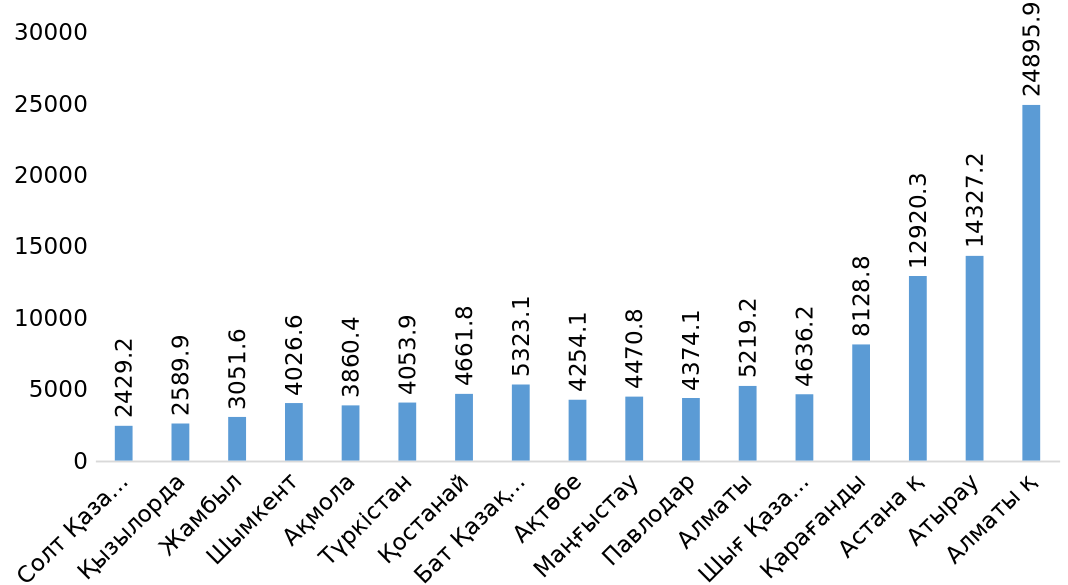
\includegraphics[width=0.6\textwidth]{media/ekon/image1000}
	\caption*{1 -- сурет. ҚР өңірлері бойынша 2023 жылғы ЖӨӨ көрсеткішін
талдау, млрд. теңге}
	\caption*{Ескерту - stat.gov.kz деректері негізінде автормен құрастырылған}
\end{figure}

\begin{multicols}{2}
Аймақтар бойынша келесі тұжырымдар жасауға болады (1-сурет). 2023 жылдың
қорытындысы бойынша Қазақстан өңірлері арасында ЖӨӨ -- нің ең жоғары
көрсеткіші Алматы қаласында - 24895,9 млрд.теңгені; Атырау облысында -
14327,2 млрд. теңгені; Қарағанды облысында -- 8128,8 млрд. теңгені;
Батыс Қазақстан облысында - 5323,1 млрд. теңгені; Астана қаласында
12920,3 млрд. теңгені құрады. Қазақстанның жоғарыда аталған өңірлері ең
үздік 5 өңірдің қатарына енді. Әрине, дәстүр бойынша бұл аймақтар
экономикалық дамуда ең дамыған болып саналады. Егер Атырау облысын
мысалға алсақ, ол Қазақстанның мұнай астанасы болып саналады. Батыс
Қазақстан және Қарағанды облыстары шикізаттық емес сипаттағы негізгі
өнеркәсіптік кәсіпорындар шоғырланған өнеркәсіптік дамыған өңірлер болып
табылады. Әрине, Қазақстанның Алматы және Астана қалалары сияқты ірі
мегаполистері отандық және шетелдік бизнес-қоғамдастық үшін өте тартымды
болып саналады. ЖӨӨ көрсеткіші бойынша Алматы қаласы Қазақстан
Республикасы өңірлерінің рейтингінде 1-орынды иеленгені бекер емес. Егер
2019 жылы ЖӨӨ көрсеткіші Алматы қаласында 13546,9 млрд. теңгені құрады,
соңғы 5 жылда айтарлықтай өсім байқалды. 2023 жылы бұл көрсеткіш 24895,9
млрд. теңге деңгейіне жетті. 2019 жылмен салыстырғанда өсім 11349 млрд.
теңгені құрады, пайыздық арақатынаста 83,7\% - дан астам.

Бұл рейтингте аутсайдерлер Қызылорда облысы болып табылады. ЖӨӨ 2023
жылы 2589,9 млрд. теңгені құрады.

Солтүстік Қазақстан облысы да Қазақстан облыстары арасында ЖӨӨ
көрсеткіші бойынша соңғы орындардың бірінде тұр. Мәселен, 2019 жылы ол
1382,3 млрд. теңгені құрады. 2023 жылы 2429,2 млрд.теңгені құрады. 2019
жылмен салыстырғанда өсім 1046,9 млрд. теңгені құрады. Егер біз 2023
және 2019 жылдардағы пайыздық өсімді талдайтын болсақ, онда бұл
көрсеткіш соңғы бес жылда 75,7\% - ға өсті. Біздің ойымызша, бұл аймақ
Қазақстан бойынша ең соңғы орында тұрса да, дамудың жақсы көрсеткішін
көрсетіп отыр.

Жамбыл облысы да ең нашар облыстардың қатарында және Қазақстанның басқа
өңірлерімен салыстырғанда ең төмен көрсеткіштерді көрсетуде. Осы
облыстың ЖӨӨ талдауы 2019 жылы 1712,8 млрд. теңгені құрағанын, 2020 жылы
жылдық көрсеткіші 1901,3 млрд. теңгені құрағанын көрсетті. Осы жылдармен
салыстырғанда өсім 188,5 млрд. теңгені құрады. 2021 жылы бұл өсу үрдісі
сақталып, 2262,7 млрд.теңгені құрады. 2023 жылы бұл көрсеткіш 3051,6
млрд. теңгеге дейін ұлғайды. 2023 жылы ауытқу 2022 жылмен салыстырғанда
366,2 млрд. теңгені құрады.
\end{multicols}

\begin{longtable}[]{|@{}
	>{\raggedright\arraybackslash}p{(\columnwidth - 14\tabcolsep) * \real{0.0601}}|
	>{\raggedright\arraybackslash}p{(\columnwidth - 14\tabcolsep) * \real{0.1819}}|
	>{\raggedright\arraybackslash}p{(\columnwidth - 14\tabcolsep) * \real{0.1213}}|
	>{\raggedright\arraybackslash}p{(\columnwidth - 14\tabcolsep) * \real{0.1213}}|
	>{\raggedright\arraybackslash}p{(\columnwidth - 14\tabcolsep) * \real{0.1213}}|
	>{\raggedright\arraybackslash}p{(\columnwidth - 14\tabcolsep) * \real{0.1213}}|
	>{\raggedright\arraybackslash}p{(\columnwidth - 14\tabcolsep) * \real{0.1213}}|
	>{\raggedright\arraybackslash}p{(\columnwidth - 14\tabcolsep) * \real{0.1516}}|@{}}
	\caption*{3 -- кесте. Өнеркәсіп өнімін (тауарларды, көрсетілетін
	қызметтерді) өндіру көлемі}\\
  \hline
  \begin{minipage}[b]{\linewidth}\raggedright
  №
  \end{minipage} & \begin{minipage}[b]{\linewidth}\raggedright
  Аймақтар
  \end{minipage} & \begin{minipage}[b]{\linewidth}\raggedright
  2019 ж.
  \end{minipage} & \begin{minipage}[b]{\linewidth}\raggedright
  2020 ж.
  \end{minipage} & \begin{minipage}[b]{\linewidth}\raggedright
  2021 ж.
  \end{minipage} & \begin{minipage}[b]{\linewidth}\raggedright
  2022 ж.
  \end{minipage} & \begin{minipage}[b]{\linewidth}\raggedright
  2023 ж.
  \end{minipage} & \begin{minipage}[b]{\linewidth}\raggedright
  Ауытқуы
  
  2023/2019
  
  +,- / \%
  \end{minipage} \\ \hline
  \endfirsthead
  \hline
  \begin{minipage}[b]{\linewidth}\raggedright
  №
  \end{minipage} & \begin{minipage}[b]{\linewidth}\raggedright
  Аймақтар
  \end{minipage} & \begin{minipage}[b]{\linewidth}\raggedright
  2019 ж.
  \end{minipage} & \begin{minipage}[b]{\linewidth}\raggedright
  2020 ж.
  \end{minipage} & \begin{minipage}[b]{\linewidth}\raggedright
  2021 ж.
  \end{minipage} & \begin{minipage}[b]{\linewidth}\raggedright
  2022 ж.
  \end{minipage} & \begin{minipage}[b]{\linewidth}\raggedright
  2023 ж.
  \end{minipage} & \begin{minipage}[b]{\linewidth}\raggedright
  Ауытқуы
  
  2023/2019
  
  +,- / \%
  \end{minipage} \\ \hline
  \endhead
  \hline
  \endfoot
  \hline
  \endlastfoot
  1 & Қазақстан Республикасы, млрд. теңге & 29380,3 & 27028,5 & 37606,2 & 48777,1 & 46991,7 & 17611,4/59,9 \\ \hline
  2 & Ақмола & 791,1 & 1040,5 & 1138,9 & 1515,0 & 1793,1 & 1002/126,6 \\ \hline
  3 & Ақтөбе & 1856,7 & 1595,5 & 2247,4 & 2827,3 & 2544,9 & 688,2/37,0 \\ \hline
  4 & Алматы & 1009,8 & 1246,5 & 1500,7 & 1651,7 & 1753,1 & 743,3/73,6 \\ \hline
  5 & Атырау & 7888,1 & 5174,8 & 8557,5 & 13341,7 & 10815,0 & 2926,9/37,1 \\ \hline
  6 & Батыс Қазақстан & 2392,1 & 1822,8 & 2843,1 & 3924,9 & 3527,1 & 1135/47,4 \\ \hline
  7 & Жамбыл & 476,9 & 518,2 & 639,1 & 881,3 & 856,2 & 379,3/79,5 \\ \hline
  8 & Қарағанды & 2620,9 & 2965,6 & 4353,6 & 3865,3 & 3531,6 & 910,7/34,7 \\ \hline
  9 & Қостанай & 1206,9 & 1541,9 & 2333,1 & 2470,1 & 2670,3 & 1463,4/121,2 \\ \hline
  10 & Қызылорда & 852,1 & 653,2 & 808,5 & 977,9 & 1043,5 & 191,4/22,4 \\ \hline
  11 & Маңғыстау & 2908,7 & 2156,4 & 2726,7 & 3182,6 & 3065,7 & 157/5,4 \\ \hline
  12 & Павлодар & 1988,9 & 2117,0 & 2783,3 & 3230,4 & 3157,6 & 1168,7/58,7 \\ \hline
  13 & Солтүстік Қазақстан & 263,5 & 315,5 & 394,6 & 519,6 & 674,8 & 411,3/156,1 \\ \hline
  14 & Түркістан & 504,9 & 543,1 & 738,2 & 907,9 & 1054,7 & 549,8/108,8 \\ \hline
  15 & Шығыс Қазақстан & 2153,9 & 2400,3 & 2763,4 & 2217,6 & 2319,9 & 166/7,7 \\ \hline
  16 & Абай & - & - & - & 1225,8 & 1597,0 & - \\ \hline
  17 & Жетісу & - & - & - & 297,3 & 325,2 & - \\ \hline
  18 & Ұлытау & - & - & - & 1036,5 & 1141,3 & - \\ \hline
  19 & Астана қ. & 884,3 & 1184,4 & 1543,9 & 1972,3 & 1933,0 & 1048,7/118,5 \\ \hline
  20 & Алматы қ. & 1001,1 & 1081,6 & 1420,7 & 1763,7 & 2096,0 & 1094,9/109,3 \\ \hline
  21 & Шымкент қ. & 579,5 & 670,5 & 812,8 & 967,2 & 1090,7 & 511,2/88,2 \\ \hline
  \multicolumn{8}{|@{}>{\raggedright\arraybackslash}p{(\columnwidth - 14\tabcolsep) * \real{1.0000} + 14\tabcolsep}|@{}}{%
  Ескерту - stat.gov.kz деректер негізінде автор құрастырған} \\ \hline
  \end{longtable}
  

\begin{multicols}{2}
Аймақтың дамуын сипаттайтын маңызды көрсеткішті қарастырайық, бұл
өнеркәсіптік өнім өндірісінің көрсеткіші болып табылады (кесте 3).

Бұл көрсеткіш облыстың өнеркәсіптік әлеуетін сипаттайды. Өйткені,
өнеркәсіп салаларын дамыту көші-қон және демографиялық мәселелер,
халықтың түрлі әлеуметтік мәселелері және т. б. сияқты көптеген
әлеуметтік мәселелерді шешуге мүмкіндік береді.

Қазақстан Республикасы бойынша өнеркәсіп өнімі өндірісінің көлемі
серпінмен өзгерді. Мәселен, 2019 жылы бұл көрсеткіш 29380,3 млрд.теңгені
құрады, 2020 жылы 27028,5 млрд.теңгені құрады. Жалпы Республика бойынша
бұл көрсеткіш 2023 жылы 2019 жылмен салыстырғанда 17611,4 млрд.теңгеге
артты (59,9 пайыз).

Өңірлер бөлінісінде 2023 жылы рейтингті дәстүрлі түрде 10815,0 млрд.
теңге көрсеткішімен Атырау облысы алады. Жалпы, Атырау облысы бірнеше
жыл қатарынан ҚР негізгі макроэкономикалық көрсеткіштері бойынша бірінші
орында тұр. Одан кейін Қарағанды өңірі 3531,6 млрд.теңге, Батыс
Қазақстан облысы -- 3527,1 млрд. теңге, Павлодар облысы -- 3157,6 млрд.
теңге. Бұдан әрі 3065,7 млрд. теңге көрсеткішімен Маңғыстау облысы және
2319,9 млрд. теңге көрсеткішімен Шығыс Қазақстан облысы орналасқан.
Бұдан кейін Ақтөбе облысы 2544,9 млрд. теңге көрсеткішімен келеді.
Қазақстан бойынша Республикалық маңызы бар қалалар арасында Астана қ.осы
көрсеткіш бойынша орташа деңгейі 1933,0 млрд. теңге, Алматы қаласы
2096,0 млрд. теңгені құрайды.

Ең нашар нәтижелерді Солтүстік Қазақстан облысы 674,8 млрд. теңге
көрсеткенін байқауға болады. Жамбыл облысында да бұл көрсеткіш деңгейі
2023 жылы 856,2 млрд. теңгені құрайды. Түркістан және Қызылорда
облыстары айтарлықтай төмен көрсеткіштерді көрсетіп отыр. Мәселен, 2023
жылы Түркістан облысында өнеркәсіп өнімін өндіру көлемі 1054,7 млрд.
теңгені, ал Қызылорда облысында 1043,5 млрд. теңгені құрады.

Аймақтың экономикалық дамуын сипаттайтын келесі маңызды
көрсеткіш-негізгі капиталға инвестициялар. Бұл өңірге инвестиция тарту
жаңа өндірістерді ашуға, соның ішінде жаңа және қосымша жұмыс орындарын
құруға ықпал ететін болады. Өз кезегінде, бұл Қазақстан Республикасының
көптеген аймақтарына мемлекеттің үдемелі экономикалық инвестициялық
саясатының арқасында белсенді түрде өз шешімін табатын әлеуметтік
аспектілерді шешуге мүмкіндік береді. Тікелей шетелдік инвестицияларды
тарту жетілдірілген технология, басқару дағдылары, ноу-хау, инновациялық
мүмкіндіктер, капиталды жинақтау және онымен байланысты физикалық
активтерді алу сияқты құнды материалдық және материалдық емес активтерді
алуға ықпал етеді {[}8{]}.
\end{multicols}


\begin{longtable}[H]{|@{}
	>{\raggedright\arraybackslash}p{(\columnwidth - 12\tabcolsep) * \real{0.1966}}|
	>{\raggedright\arraybackslash}p{(\columnwidth - 12\tabcolsep) * \real{0.1213}}|
	>{\raggedright\arraybackslash}p{(\columnwidth - 12\tabcolsep) * \real{0.1213}}|
	>{\raggedright\arraybackslash}p{(\columnwidth - 12\tabcolsep) * \real{0.1213}}|
	>{\raggedright\arraybackslash}p{(\columnwidth - 12\tabcolsep) * \real{0.1213}}|
	>{\raggedright\arraybackslash}p{(\columnwidth - 12\tabcolsep) * \real{0.1213}}|
	>{\raggedright\arraybackslash}p{(\columnwidth - 12\tabcolsep) * \real{0.1971}}|@{}}
	\caption*{4 -- кесте. ҚР өңірлері бөлінісінде негізгі капиталға
	инвестициялар көлемі}\\
	\hline
  \textbf{Аймақтар} & \textbf{2019 ж.} & \textbf{2020 ж.} & \textbf{2021 ж.} & \textbf{2022 ж.} & \textbf{2023 ж.} & \textbf{Ауытқуы 2023/2019 +,- / \%} \\
  \hline
  \endfirsthead
  \hline
  \textbf{Аймақтар} & \textbf{2019 ж.} & \textbf{2020 ж.} & \textbf{2021 ж.} & \textbf{2022 ж.} & \textbf{2023 ж.} & \textbf{Ауытқуы 2023/2019 +,- / \%} \\
  \hline
  \endhead
  \hline
  \endfoot
  \hline
  \endlastfoot
  Қазақстан Республикасы, млрд. теңге & 12576,7 & 12270,1 & 13242,2 & 15251,1 & 17649,3 & 5072,6/40,3 \\
  Ақмола & 333,7 & 436,6 & 514,6 & 579,9 & 613,5 & 279,8/83,8 \\
  Ақтөбе & 598,8 & 648,0 & 817,1 & 960,1 & 1025,7 & 426,9/71,2 \\
  Алматы & 647,3 & 682,4 & 733,4 & 613,9 & 737,7 & 90,4/13,9 \\
  Атырау & 4328,2 & 3178,9 & 2910,1 & 3003,5 & 2934,8 & -1393,4/-32,1 \\
  Батыс Қазақстан & 586,2 & 481,4 & 428,7 & 537,8 & 675,2 & 89/15,1 \\
  Жамбыл & 296,3 & 350,0 & 398,6 & 428,5 & 536,5 & 240,2/81,0 \\
  Қарағанды & 811,4 & 692,3 & 796,8 & 724,9 & 876,5 & 65,1/8,1 \\
  Қостанай & 288,7 & 336,5 & 431,1 & 492,0 & 561,6 & 272,9/94,5 \\
  Қызылорда & 400,2 & 292,3 & 308,9 & 413,2 & 513,7 & 113,5/28,3 \\
  Маңғыстау & 556,5 & 582,2 & 629,1 & 785,7 & 1102,1 & 545,6/98,1 \\
  Павлодар & 494,6 & 487,1 & 571,9 & 742,7 & 797,4 & 302,8/61,2 \\
  Солтүстік Қазақстан & 234,4 & 286,2 & 333,1 & 368,4 & 443,6 & 209,2/89,2 \\
  Түркістан & 443,5 & 705,7 & 659,1 & 742,5 & 948,8 & 505,3/113,9 \\
  Шығыс Қазақстан & 621,9 & 729,1 & 834,0 & 555,2 & 648,6 & 26,7/4,3 \\
  Абай & - & - & - & 414,4 & 527,3 & - \\
  Жетісу & - & - & - & 291,8 & 356,7 & - \\
  Ұлытау & - & - & - & 175,4 & 228,9 & - \\
  Астана қ. & 919,1 & 1125,2 & 1225,0 & 1462,5 & 1655,0 & 735,9/80,0 \\
  Алматы қ. & 820,4 & 976,7 & 1187,6 & 1407,9 & 1803,1 & 982,7/119,7 \\
  Шымкент қ. & 194,9 & 278,7 & 462,4 & 549,6 & 661,7 & 466,8/239,5 \\
  \multicolumn{7}{|@{}>{\raggedright\arraybackslash}p{(\columnwidth - 12\tabcolsep) * \real{1.0000} + 12\tabcolsep}|@{}}{%
  Ескерту - stat.gov.kz деректер негізінде автор құрастырған} \\
  \end{longtable}

\begin{multicols}{2}
Қазақстан Республикасы бойынша негізгі капиталға инвестициялар көлемі
2019 жылы 12576,7 млрд. теңгені құрады, ал 2020 жылы бұл көрсеткіш
азайып, 12270,1 млрд.теңгені құрады. 2020 жылы инвестициялық жобалардың
көпшілігі пандемияға байланысты қатып қалды немесе белгісіз мерзімге
кейінге қалдырылды. 2021 жылы Қазақстан экономикасы қалпына келе
бастады, онда экономиканың барлық салаларында экономикалық даму
индикаторлары тұтастай өсе бастады. 2021 жылы инвестиция көлемі бойынша
өсім 13242,2 млрд. теңгені құрады. Бұл жағдайда бұл көрсеткіштің
айтарлықтай өсуі байқалады, ол 972,1 млрд. теңгені құрады. 2023 жылы
2022 жылға қарағанда 2398,2 млрд. теңгеге артты.
\end{multicols}



\begin{figure}[H]
	\centering
	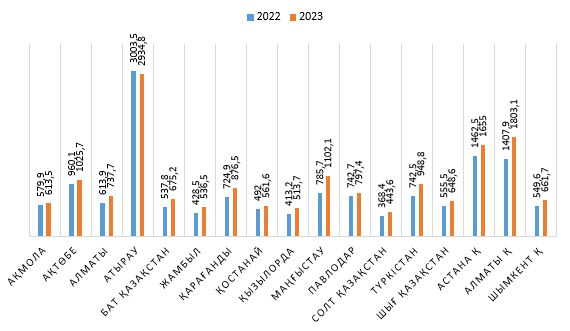
\includegraphics[width=0.6\textwidth]{media/ekon/image1.3}
	\caption*{2 -- сурет. 2022-2023 жж. ҚР өңірлері бойынша негізгі капиталға
	инвестициялар көлемінің серпіні, млрд. теңге}
	\caption*{Ескерту - stat.gov.kz деректер негізінде автор құрастырған}
\end{figure}

\begin{multicols}{2}
Өңірлер бойынша негізгі капиталға инвестициялар көлемінің динамикасын
талдау мыналарды көрсетті. 2022-2023 жылдар кезеңінде өңірлер арасында
сенімді бірінші орынды Атырау өңірі алады, онда негізгі капиталға
инвестициялар көлемі 2022 жылы -- 3003,5 млрд.теңге, ал келесі 2023 жылы
керісінше осы көрсеткіш бойынша төмендеу орын алды, ол 2934,8 млрд.
теңгені құрады. Бұл жағдайда ауытқу 68,7 млрд. теңгені құрады. Өңірдегі
инвестициялардың жалпы көлемінің қысқаруының себебі -- өнеркәсіпке
салымдардың күрт төмендеуі салдарынан болып отыр. Өңір өнеркәсібінің
негізгі бағыты «шикі мұнай және табиғи газ өндіру» болып табылады.
Атырау облысының мұнай-газ секторына жоғары тәуелділігі өңірді әлемдік
энергетика нарығындағы өзгерістерге осал етеді. Мұнай бағасының
төмендеуі осы салада жұмыс істейтін компаниялардың кірістерін
төмендетеді, бұл өз кезегінде өндірісті дамытуға және модернизациялауға
инвестиция көлемін азайтады.

Бұдан әрі негізгі капиталға инвестициялар тарту бойынша үздік өңірлердің
тізімін ірі іскерлік орталық -- Алматы қаласы алады, 2022 жылы
көрсеткіші 1407,9 млрд.теңге, 2023 жылы 1803,1 млрд. теңгені құрады.
Жоғарыда көрсетілген сандардан Алматы қаласы бойынша бұл көрсеткіштің
артып келе жатқанын байқауға болады. Өсім салыстырмалы түрде 128\%
құрады.

Инвестициялар көлемі деңгейі бойынша рейтингте келесі орынды Астана
қаласы алады. 2022 жылы бұл көрсеткіштің мәні 1462,5 млрд.теңгені, 2023
жылы 1655,0 млрд. теңгені құрады. Берілген сандар бойынша осы
көрсеткіштің тұрақты өсуін байқауға болады, өсім 113,1\% құрады.

Бұдан әрі негізінен өнеркәсіптік өңірлер орналасқан аймақтар алады, олар
Шығыс Қазақстан облысы, Қарағанды облысы, Маңғыстау облысы, Алматы
облысы, Ақмола облысы және т.б.

Инвестиция тарту бойынша ең төмен нәтижелерді Солтүстік Қазақстан облысы
көрсетеді. Мәселен, осы өңірде негізгі қаражатқа инвестициялар тарту
көрсеткіші 2022 жылы 368,4 млрд.теңгені құрады, 2023 жылы бұл көрсеткіш
443,6 млрд.теңгеге дейін ұлғайды. Салыстырмалы түрде өсім 120,4\%
құрады. Біздің ойымызша, бұл жақсы нәтиже және біз бұл аймақтың қазіргі
уақытта өте қарқынды дамып келе жатқанын көріп отырмыз.
\end{multicols}


\begin{longtable}[]{|@{}>{\raggedright\arraybackslash}p{(\columnwidth - 12\tabcolsep) * \real{0.2117}}|
	>{\raggedright\arraybackslash}p{(\columnwidth - 12\tabcolsep) * \real{0.1213}}|
	>{\raggedright\arraybackslash}p{(\columnwidth - 12\tabcolsep) * \real{0.1061}}|
	>{\raggedright\arraybackslash}p{(\columnwidth - 12\tabcolsep) * \real{0.1213}}|
	>{\raggedright\arraybackslash}p{(\columnwidth - 12\tabcolsep) * \real{0.1061}}|
	>{\raggedright\arraybackslash}p{(\columnwidth - 12\tabcolsep) * \real{0.1213}}|
	>{\raggedright\arraybackslash}p{(\columnwidth - 12\tabcolsep) * \real{0.2123}}|@{}}
	\caption*{5 -- кесте. Халықтың жан басына шаққандағы орташа номиналды
	ақшалай кірістерін бағалау}\\
	\hline
\multirow{2}{=}{\begin{minipage}[b]{\linewidth}\raggedright Аймақтар\end{minipage}} &
\multicolumn{5}{|>{\raggedright\arraybackslash}p{(\columnwidth - 12\tabcolsep) * \real{0.5760} + 8\tabcolsep}|}{%
\begin{minipage}[b]{\linewidth}\raggedright орташа жан басына шаққанда, теңге\end{minipage}} &
\multirow{2}{=}{\begin{minipage}[b]{\linewidth}\raggedright Ауытқуы 2023/2019 +,- / \%\end{minipage}} \\ 
& \begin{minipage}[b]{\linewidth}\raggedright 2019 ж.\end{minipage} & 
\begin{minipage}[b]{\linewidth}\raggedright 2020 ж.\end{minipage} & 
\begin{minipage}[b]{\linewidth}\raggedright 2021 ж.\end{minipage} & 
\begin{minipage}[b]{\linewidth}\raggedright 2022 ж.\end{minipage} & 
\begin{minipage}[b]{\linewidth}\raggedright 2023 ж.\end{minipage} \\ 
\hline
\endhead
\hline
\endfoot
\hline
Қазақстан Республикасы & 104282 & 116126 & 130616 & 164438 & 189953 & 85671/82,1 \\
Ақмола & 91933 & 107224 & 122039 & 151345 & 168301 & 76368/83,1 \\
Ақтөбе & 92696 & 98360 & 115009 & 142531 & 163509 & 70813/76,3 \\
Алматы & 79528 & 86606 & 101709 & 124587 & 131885 & 52357/65,8 \\
Атырау & 212571 & 215076 & 251597 & 291852 & 319998 & 107427/50,5 \\
Батыс Қазақстан & 107202 & 112319 & 128077 & 151855 & 172089 & 64887/60,5 \\
Жамбыл & 70330 & 80516 & 90255 & 112952 & 129051 & 58721/83,5 \\
Қарағанды & 106481 & 130552 & 140164 & 172498 & 208453 & 101972/95,7 \\
Қостанай & 92543 & 105856 & 124221 & 156124 & 178837 & 86294/93,2 \\
Қызылорда & 76971 & 85142 & 92531 & 120896 & 136698 & 59727/77,5 \\
Маңғыстау & 137539 & 141506 & 156740 & 200232 & 231263 & 93724/68,1 \\
Павлодар & 106226 & 119334 & 138244 & 181426 & 199404 & 93178/87,7 \\
Солтүстік Қазақстан & 88229 & 103292 & 117275 & 156386 & 178495 & 90266/102,3 \\
Түркістан & 52650 & 63443 & 69103 & 90078 & 103735 & 51085/97,0 \\
Шығыс Қазақстан & 97835 & 111632 & 133689 & 183500 & 208691 & 110856/113,3 \\
Абай & - & - & 116776 & 139511 & 164138 & - \\
Жетісу & - & - & 91986 & 114873 & 127875 & - \\
Ұлытау & - & - & 162387 & 204233 & 263693 & - \\
Астана қ. & 162400 & 174396 & 194398 & 238677 & 272742 & 110342/67,9 \\
Алматы қ. & 150380 & 164721 & 179554 & 238496 & 288339 & 137959/91,7 \\
Шымкент қ. & 70202 & 75725 & 81714 & 102796 & 120218 & 50016/71,2 \\
\hline
\multicolumn{7}{|>{\raggedright\arraybackslash}p{(\columnwidth - 12\tabcolsep) * \real{1.0000} + 12\tabcolsep}|}{%
Ескерту - stat.gov.kz деректер негізінде автор құрастырған} \\
\end{longtable}


\begin{multicols}{2}
Кесте мәліметтерін талдайтын болсақ, халықтың жан басына шаққандағы
орташа номиналды ақшалай кірістері Атырау және Маңғыстау облыстарында
жоғары мәнге ие, яғни 319998 және 231263 теңгені құрайды. Дәстүрлі түрде
мұнай ресурстарына бай аймақ дамыған мұнай-газ секторының және осы
саладағы жоғары жалақының арқасында көшбасшылықты сақтауды жалғастыруда.
Одан кейінгі орында Астана және Алматы қалалары алады, 272742 және
288339 теңгені құрайды.

Аймақтар арасындағы аутсайдер болып Түркістан облысы орналасқан, онда
жан басына шаққандағы орташа табыс небәрі 103735 теңгені құрайды. Бұл
республика бойынша орташа көрсеткіштерден екі есе аз. Түркістан облысы
ауыл шаруашылығы бағытымен және өнеркәсіптік даму деңгейінің
төмендігімен жергілікті халықтың табыс деңгейіне әсер ететін баяу
экономикалық өсіммен бетпе-бет келеді.

Тұрақты даму тұжырымдамасы үш өлшемге негізделген. Аймақтардың дамуы,
әдетте, белгілі бір аумақтағы қоғамдастықтың (әлеуметтік, экономикалық,
экологиялық және денсаулық сақтау, технологиялық, мәдени және
рекреациялық) интегралды дамуы ретінде анықталады. Аймақтың дамуы
олардың оңтайлы кеңеюіне негізделуі керек құрамдас бөліктер (әлеуметтік,
табиғи және экономикалық даму аспектілері) өмірдің белгілі бір деңгейін
ұстап тұруға және аталған құрамдас бөліктер арқылы сапаны жақсартуға
бағытталған. Өңірлік даму белгілі бір аумақтағы дәстүрлі саясатты ғана
емес, сонымен бірге нақты саяси және мәдени контексте ұйымдастырылған
әлеуметтік-экономикалық процесті де қамтиды. Бүгінгі контекстегі
аймақтық даму көптеген дағдарыстар (қаржылық, азық-түлік және
энергетика) бізді қазіргі заманның экономикалық парадигмасын қайта
қарауға және қазіргі уақытта болашақ ұрпаққа жұмыспен қамту, әлеуметтік
прогресс, өмір сапасы және табиғатты құрметтеу салаларында қалдыратын
орындалмаған уәделерді қалай жақсырақ орындау керектігін бағалауға
мәжбүр ететін маңызды кезеңде. Орнықты даму тіректерін өңірлік деңгейге
интеграциялаудың маңыздылығына күмән жоқ болса да, бұл тұжырымдаманы
іске асыру іс жүзінде күрделі міндет болып шықты. Шын мәнінде, тұрақты
дамудың экологиялық, экономикалық және әлеуметтік өлшемдерін аймақтық
деңгейде интеграциялау әр түрлі салаларда бірін-бірі толықтыратын және
үйлестірілген іс-әрекеттерді жүзеге асыруды көздейді, бұл экономикалық
өсуге алып келеді, сонымен қатар әлеуметтік мақсаттарға қол жеткізуге
мүмкіндік береді. Осы үш өлшемнің тиімді интеграциясы бір-бірін
толықтыратын және тұрақты дамудың жан-жақты шеңберіне сәйкес келетін
бағытталған және нақты іс-шаралар кешенін жүзеге асыруды талап етеді
{[}9{]}.

Мысалы, өнеркәсіптік даму деңгейі жоғары аймақтарға белсенді бейімделу
моделі тән болды, ол өз күштерін пайдалану стратегиясына, нарыққа жедел
ілгерілеуді қамтамасыз ететін инновациялық, дәстүрлі емес әдістер мен
ынталандыруларды таба білуге бағытталған. Тұрақты дамуға бейімделу
коэффициентін анықтау үшін келесі көрсеткіштерді есептеуге болады.

Орнықты дамуға бейімделудің өңірлік коэффициенті математикалық, дәлірек
айтқанда, өңірдің жан басына шаққандағы жалпы өңірлік өнімінің
республика халқының жан басына шаққандағы жалпы өңірлік өнімге қатынасы
ретінде есептелді. Ұсынылған есептік көрсеткіш-бұл салыстырмалы
бейімделудің аймақтық коэффициенті, ол интеграцияланған түрде аймақтың
даму дәрежесін, сондай-ақ белгілі бір аумақта экономиканың тиімділігі
мен күрделілігін көрсетеді. Сонымен, тұрақтылыққа салыстырмалы
бейімделудің аймақтық коэффициенті:

\[C_{(ra)} = \frac{{GRP}_{pcreg}}{{GRP}_{pcrep}}\]

Мұнда:

\({GRP}_{pcreg} - \ аймақтың\) жан басына шаққандағы жалпы өңірлік
өнімі;

\({GRP}_{pcrep}\  - \ \)республиканың жан басына шаққандағы жалпы
өңірлік өнімі {[}10{]}.

Осы есептеу бойынша аймақтық коэффициент 6 кестеде көрсетілген.
\end{multicols}


\begin{longtable}[]{|@{}>{\raggedright\arraybackslash}p{(\columnwidth - 6\tabcolsep) * \real{0.3330}}|
	>{\raggedright\arraybackslash}p{(\columnwidth - 6\tabcolsep) * \real{0.2122}}|
	>{\raggedright\arraybackslash}p{(\columnwidth - 6\tabcolsep) * \real{0.2123}}|
	>{\raggedright\arraybackslash}p{(\columnwidth - 6\tabcolsep) * \real{0.2425}}|@{}}
	\caption*{6 -- кесте. 2021-2023 жылдарға арналған тұрақты дамуға
	бейімделуге қатысты аймақтық коэффициенті}\\
	\hline
\begin{minipage}[b]{\linewidth}\raggedright Аймақтар\end{minipage} &
\begin{minipage}[b]{\linewidth}\raggedright 2021 ж.\end{minipage} &
\begin{minipage}[b]{\linewidth}\raggedright 2022 ж.\end{minipage} &
\begin{minipage}[b]{\linewidth}\raggedright 2023 ж.\end{minipage} \\ 
\endhead
\hline
\endfoot
\hline
Ақмола & 0,82503 & 0,83797 & 0,81372 \\
Ақтөбе & 0,90135 & 0,90604 & 0,75672 \\
Алматы & 0,49822 & 0,54117 & 0,57091 \\
Атырау & 3,63010 & 3,77957 & 3,40661 \\
Батыс Қазақстан & 1,20501 & 1,22386 & 1,28014 \\
Жамбыл & 0,44747 & 0,41859 & 0,41533 \\
Қарағанды & 1,22667 & 1,21347 & 1,18949 \\
Қостанай & 0,92415 & 0,94890 & 0,93169 \\
Қызылорда & 0,53081 & 0,55213 & 0,51347 \\
Маңғыстау & 1,12417 & 1,10086 & 0,95578 \\
Павлодар & 1,17363 & 1,10758 & 0,96304 \\
Солтүстік Қазақстан & 0,75008 & 0,77538 & 0,75830 \\
Түркістан & 0,30853 & 0,31634 & 0,31602 \\
Шығыс Қазақстан & 0,84271 & 1,01307 & 1,05686 \\
Астана қ. & 1,66638 & 1,52398 & 1,54135 \\
Алматы қ. & 1,69668 & 1,70029 & 1,88368 \\
Шымкент қ. & 0,55295 & 0,52952 & 0,55406 \\
\hline
\multicolumn{4}{|>{\raggedright\arraybackslash}p{(\columnwidth - 6\tabcolsep) * \real{1.0000} + 6\tabcolsep}|}{%
Ескерту - stat.gov.kz деректер негізінде автор құрастырған} \\
\hline
\end{longtable}


\begin{multicols}{2}
Өңірлердің тұрақты даму талаптарына бейімделу дәрежесін анықтау күрделі
мәселелердің бірі болып табылады, ол екеуін де біріктіруді қажет етеді:
сандық және сапалық тәсілдер. Оның зерттеу нысаны аймақтың
әлеуметтік-экономикалық әлеуеті болғандықтан, оны пайдалану тұтастай
республика экономикасын реформалау барысымен анықталады. Аймақтың
әлеуметтік-экономикалық әлеуеті жалпы қоғамда болып жатқан терең сандық
және сапалық өзгерістерге байланысты.

Әлеуметтік-экономикалық әлеуеттің аймақтық көрінісі:

- экономикалық, әлеуметтік және экологиялық дамудың күрделілігі;

- табиғатты пайдалану және қоршаған ортаны қорғау қоғамдастығының
міндеттері;

- аумақтық өндірістік қоғамдастық;

- халықтың салыстырмалы тұрақтылығы және елді мекендер жүйесінің
бірлігі;

- аумақта жұмыс істейтін өндірістік, әлеуметтік және нарықтық
инфрақұрылымның бірлігі.

Тұрақты дамуға бейімделудің өңірлік коэффициентін бағалау 2021-2023
жылдар аралығында Атырау облыстары мен Астана және Алматы қалалары
тұрақты түрде көш бастап тұрғанын көрсетті. Осылайша, Жамбыл және
Түркістан облыстары ең төменгі көрсеткішті көрсетіп отыр.

{\bfseries Қорытынды.} Аймақтық дамуды мемлекеттік басқару саласындағы
зерттеулер аймақтық саясаттың әр түрлі басым бағыттарын бөліп көрсетеді,
олардың таңдауы көбінесе белгілі бір даму сценарийіне сәйкес келеді.

Қазақстан аймақтарының әлеуметтік-экономикалық жағдайы бүгінгі таңда
олардың дамуында белгілі бір теңгерімсіздіктер орын алатындай дамыды.
Олардың кейбіреулері айтарлықтай даму қарқынына ие және тұрақты оң
динамика байқалады. Өнеркәсіптік қалаларда экономикалық көрсеткіштер
жақсы нәтиже көрсетеді, бірақ кірістер мен шығыстардың өмір сүру деңгейі
артта қалған аймақтарға ұқсас, елдің оңтүстігінде орналасқан аймақтар
төмен макроэкономикалық көрсеткіштерді көрсетеді, бірақ шағын және орта
бизнесті дамытуда көшбасшы болып табылады. Бұл жоғары кәсіпкерлік
факторға қатысты. Өнеркәсіптік қалаларда халықтың 80\%-дан астамы
жалдамалы жұмысшылар болса, өнеркәсіптік емес қалаларда халық шағын және
орта бизнеспен айналысады.

Республика өңірлерінде жұмыссыздық деңгейі, тұтыну бағаларының индексі
және тұтыну үшін пайдаланылатын табысы ең төменгі күнкөріс деңгейінен
төмен халықтың үлесі айтарлықтай қарқынмен төмендеуде. Сондай-ақ,
көптеген кезеңдерде инфляция деңгейі ақшалай кірістердің номиналды
индексінің өсуінен төмен, яғни халықтың нақты кірістерінің өсуі
байқалады.

Аймақтық экономиканы тұрақты дамуға бейімдеу экономиканы бәсекеге
қабілетті деңгейге жеткізу стратегиясын таңдау және әлеуметтік
салалардың дамуындағы айырмашылықтарды азайту, яғни халықтың өмір сүру
деңгейін теңестіру сияқты өзара байланысты екі мәселені шешуді талап
етеді. Аймақтардағы объективті айырмашылықтар оларды дамыту
стратегияларын әзірлеуде сараланған тәсілдерді қажет етеді. Осы тұрғыдан
алғанда, шешімі жан-жақты жүзеге асырылуы тиіс проблемалық аймақтардың
кластерлерін анықтау.

Аймақтың экономикалық әлеуетін анықтау мақсатында біз тұрақты дамуға
бейімделудің аймақтық коэффициентін есептедік, онда көрсеткіштері төмен
аймақтар анықталды, олар Түркістан және Жамбыл облыстары. Бұл аймақтар
көптеген макроэкономикалық көрсеткіштер бойынша артта қалғанын көрсетсе
де, бұл аймақтар шағын және орта кәсіпкерліктің белсенділігі бойынша көш
бастап тұр. Экономиканың негізгі қозғаушы күші шағын және орта бизнес
екені белгілі.

Аймақтардағы объективті айырмашылықтар оларды дамыту стратегияларын
әзірлеуде сараланған тәсілдерді қажет етеді. Аймақтық экономиканы
тұрақты дамуға бейімдеу өзара байланысты екі мәселені шешуді талап
етеді, мысалы, экономиканы бәсекеге қабілетті деңгейге жеткізу
стратегиясын таңдау және халықтың өмір сүру деңгейін теңестіру үшін
әлеуметтік салалардың дамуындағы айырмашылықтарды азайту. Осы тұрғыдан
алғанда, осы міндеттерді шешу кешенді түрде жүзеге асырылуы тиіс
проблемалық аймақтардың кластерлерін анықтау қажет сияқты.
\end{multicols}

\begin{center}
{\bfseries Әдебиеттер}
\end{center}

\begin{references}
1.Кузнецов А. П. Устойчивое развитие региона: эколого-экономические
аспекты:

монография / Кузнецов А.П., Селименков Р.Ю.; под науч. рук. д-ра экон.
наук, проф. Усковой Т.В. -- Вологда: ИСЭРТ РАН, 2015. -- 136 с. ISBN
978-5-93299-306-4

2.Жангирова Р.Н. Возможности и условия устойчивого развития аграрной
отрасли

Республики Казахстан // Вестник университета «Туран». -2020. -№3 (87).
С. 78-83. DOI: 10.46914/1562-2959-2020-1-3-78-83

3.Стеблянская А.Н., Ванг Дж., Габдрахманова Н.Т., Алероев У.А. Системная

трансформация экофинансовой модели устойчивого роста (на примере
китайских и российских нефтегазовых компаний) // Вестник Московского
университета. Серия 6. Экономика. -2019. -№4. URL:
\href{https://cyberleninka.ru/article/n/sistemnaya-transformatsiya-ekofinansovoy-modeli-ustoychivogo-rosta-na-primere-kitayskih-i-rossiyskih-neftegazovyh-kompaniy}{https://cyberleninka.ru}
(қаралған күні: 14.10.2024).

4.Кириллов С.Н., Молоткова Е.Г. Факторы устойчивого развития региона //
Юг России:

экология, развитие. -2010. --Т. 5(4). --С. 20-22. DOI:
10.18470/1992-1098-2010-4-20-22

5.Аникина И.Д., Аникин А.А. Эколого-экономическое состояние регионов:

совершенствование методологии и методики оценки // Вестник ВолГУ. Серия
3: Экономика. Экология. -2019. -№4. --P. 141-151. DOI:
10.15688/ek.jvolsu.2019.4.14

6.Барташевич А.А. Формирование механизма регионального устойчивого
развития на базе

управления эколого - экономическими рисками (на материалах Карачаево -
Черкесской республики): автореф. дис. \ldots канд. экон. наук: 08.00.05-
Майкоп, 2012. -- 28 с.

7.Малдыбаева Г. Валовый региональный продукт: оценка развития территорий

//Ежеквартальный научно -- информационный журнал Экономика и статистика
- 3/2017 год. - С.4-10.

8.Ыдырыс С.С., Шарханова Б. Прямые иностранные инвестиции в странах
центральной

Азии: лидеры, способы привлечения, перспективы // Вестник КазУЭФиМТ.
-№1(46) /2022. -- С. 178-185. DOI:10.52260/2304-7216.2022.1(46).23

9.Sandra C. Valencia, David Simon, Sylvia Croese, Joakim Nordqvist,
Michael Oloko, Tarun

Sharma, Nick Taylor Buck \& Ileana Versace Adapting the Sustainable
Development Goals and the New Urban Agenda to the city level: Initial
reflections from a comparative research project // International Journal
of Urban Sustainable Development. -2019. --P. 4-23. DOI:
10.1080/19463138.2019.1573172

10. Khajieva, G. Problems of socio-economic development of
Kazakhstan' s regions in the

context of adaptation to the sustainable development / G. Khajieva, A.
Omir // Экономика: стратегия и практика. -- 2020. -- Vol. 15, No. 2. --
P. 175-186.
\end{references}

\begin{center}
{\bfseries References}
\end{center}

\begin{references}
1. Kuznecov A. P. Ustojchivoe razvitie regiona: jekologo-jekonomicheskie
aspekty: monografija / Kuznecov A.P., Selimenkov R.Ju.; pod nauch. ruk.
d-ra jekon. nauk, prof. Uskovoj T.V. -- Vologda: ISJeRT RAN, 2015. --
136 s. ISBN 978-5-93299-306-4 {[}in Russian{]}

2. Zhangirova R.N. Vozmozhnosti i uslovija ustojchivogo razvitija
agrarnoj otrasli Respubliki Kazahstan // Vestnik universiteta «Turan».
-2020. -№3 (87). S. 78-83. DOI: 10.46914/1562-2959-2020-1-3-78-83 {[}in
Russian{]}

3. Stebljanskaja A.N., Vang Dzh., Gabdrahmanova N.T., Aleroev U.A.
Sistemnaja transformacija jekofinansovoj modeli ustojchivogo rosta (na
primere kitajskih i rossijskih neftegazovyh kompanij) // Vestnik
Moskovskogo universiteta. Serija 6. Jekonomika. -2019. -№4. URL:
\href{https://cyberleninka.ru/article/n/sistemnaya-transformatsiya-ekofinansovoy-modeli-ustoychivogo-rosta-na-primere-kitayskih-i-rossiyskih-neftegazovyh-kompaniy}{https://cyberleninka.ru}
(date of review:: 14.10.2024). {[}in Russian{]}

4. Kirillov S.N., Molotkova E.G. Faktory ustojchivogo razvitija regiona
// Jug Rossii: jekologija, razvitie. -2010. --T. 5(4). --S. 20-22. DOI:
10.18470/1992-1098-2010-4-20-22 {[}in Russian{]}

5. Anikina I.D., Anikin A.A. Jekologo-jekonomicheskoe sostojanie
regionov: sovershenstvovanie metodologii i metodiki ocenki // Vestnik
VolGU. Serija 3: Jekonomika. Jekologija. -2019. -№4. --P. 141-151. DOI:
10.15688/ek.jvolsu.2019.4.14 v

6. Bartashevich A.A. Formirovanie mehanizma
regional' nogo ustojchivogo razvitija na baze upravlenija
jekologo -

jekonomicheskimi riskami (na materialah Karachaevo -
Cherkesskoj respubliki): avtoref. dis. \ldots kand. jekon. nauk:
08.00.05- Majkop, 2012. -- 28 s. {[}in Russian{]}

7. Maldybaeva G. Valovyj regional' nyj produkt: ocenka
razvitija territorij //Ezhekvartal' nyj nauchno --
informacionnyj zhurnal Jekonomika i statistika - 3/2017 god. - S.4-10.
{[}in Russian{]}

8. Ydyrys S.S., Sharhanova B. Prjamye inostrannye investicii v stranah
central' noj Azii: lidery, sposoby privlechenija,
perspektivy // Vestnik KazUJeFiMT. -№1(46) /2022. -- S. 178-185.
DOI:10.52260/2304-7216.2022.1(46).23 {[}in Russian{]}

9. Sandra C. Valencia, David Simon, Sylvia Croese, Joakim Nordqvist,
Michael Oloko, Tarun Sharma, Nick Taylor Buck \& Ileana Versace Adapting
the Sustainable Development Goals and the New Urban Agenda to the city
level: Initial reflections from a comparative research project //
International Journal of Urban Sustainable Development. -2019. --P.
4-23.

DOI: 10.1080/19463138.2019.1573172

10. Khajieva, G. Problems of socio-economic development of
Kazakhstan' s regions in the context of adaptation to the
sustainable development / G. Khajieva, A. Omir // Jekonomika: strategija
i praktika. -- 2020. -- Vol. 15, No. 2. -- P. 175-186.
\end{references}

\begin{authorinfo}
\hspace{1em}\emph{{\bfseries Авторлар туралы мәлімет}}

Батцэнгэл Хуухээ - экономика ғылымдарының докторы, профессор, Қазіргі
заманғы зерттеулер институтының директоры, Моңғол жоғары оқу орнынан
кейінгі білім беру университеті, Моңголия, е-mail:
\href{mailto:battsengel1@mail.ru}{\nolinkurl{battsengel1@mail.ru}};

Касымова С.Б. - «Экономика және басқару» кафедрасының аға оқытушысы,
магистр, Қ.Құлажанов атындағы Қазақ технология және бизнес университеті,
е-mail: \href{mailto:Sanim_81@list.ru}{\nolinkurl{Sanim\_81@list.ru}};

Мустафаев К.С. -- э.ғ.к., қауымд профессор, Қ.Құлажанов атындағы Қазақ
технология және бизнес университеті, е-mail:
\href{mailto:astana_kzo@mail.ru}{\nolinkurl{astana\_kzo@mail.ru}}.

\hspace{1em}\emph{{\bfseries Information about the author}}

Battsengel Khukhe -- Doctor of Economics, Professor, Director of the
Institute of Modern Studies, Graduate University of Mongolia, е-mail:
\href{mailto:battsengel1@mail.ru}{\nolinkurl{battsengel1@mail.ru}};

Kassymova S.B. - Master' s degree, Senior Lecturer of the
Department of Economics and Management, K.Kulazhanov Kazakh University
of Technology and Business, е-mail:
\href{mailto:Sanim_81@list.ru}{\nolinkurl{Sanim\_81@list.ru}};

Mustafayev K.S. -- Candidate of Economics, Assoc Professor, K.Kulazhanov
Kazakh University of Technology and Business, е-mail:
\href{mailto:astana_kzo@mail.ru}{\nolinkurl{astana\_kzo@mail.ru}}.
\end{authorinfo}
